
\begin{frame}
    \frametitle{Présentation}
    \begin{block}{Définitions}
	\begin{itemize}
	\item \textbf{Gestion de portefeuille :}
	      \begin{itemize}
	      \item Gérer des capitaux sous certaines contraintes
	      \item Choisir une stratégie d'investissement
	      \end{itemize}
	\item \textbf{Différents risques :}
	      \begin{itemize}
	      \item Financiers : marché, crédit, liquidité
	      \item Non financiers : modèle, perte extrême
	      \end{itemize}
	\item \textbf{Profils de rique :}
	      \begin{itemize}
	      \item Risk adverse
	      \item Risk neutral
	      \item Risk lovers/seekers
	      \end{itemize}
	\end{itemize}
    \end{block}


\end{frame}

\begin{frame}
    \frametitle{Actifs risqués}
	  \begin{figure}
	      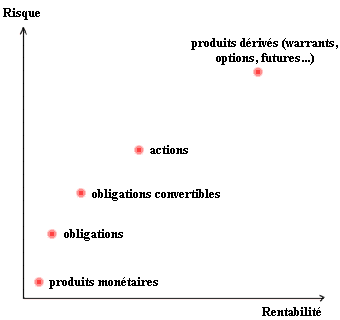
\includegraphics[scale=0.5]{images/actifsRisques.png}   
	  \end{figure}   
\end{frame}


\begin{frame}
    \frametitle{Diversification} 
      \begin{block}{Intérêts}
	\begin{enumerate}
	  \begin{columns}
	    \begin{column}{4cm}
	      \item Eviter les catastrophes
	    \end{column}
	    \begin{column}{4cm}
	      \item Réduire le risque	   
	    \end{column}
	  \end{columns}
	\end{enumerate}
      \end{block}
      \begin{figure}
	  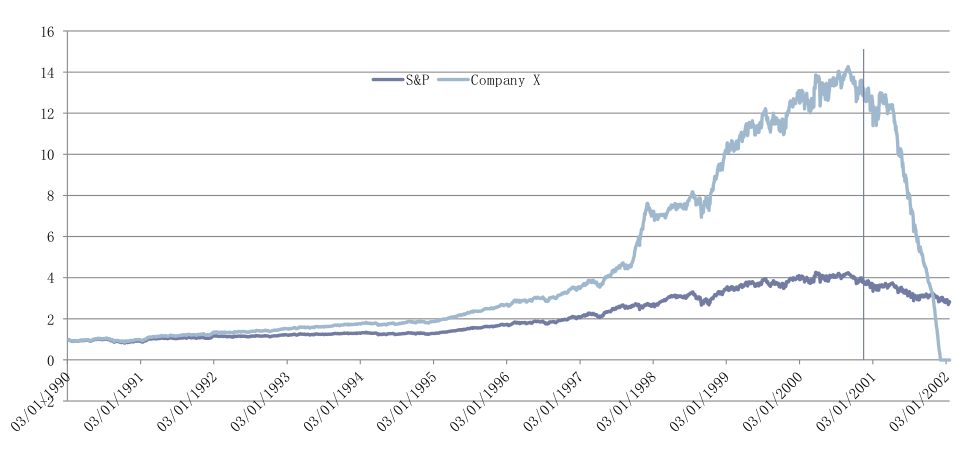
\includegraphics[scale=0.2]{images/exempleChuteEntreprise.png}   
	  \caption{Exemple d'un portefeuille à un actif (courbe bleu ciel)}
      \end{figure}  
\end{frame}



\begin{frame}
    \frametitle{Le rendement} 
    \begin{block}{Rendement d'un actif}
	\begin{itemize}
	 \item Arithmétique :  $R_{i} = \frac{1}{T} \sum_{t=1}^T R_{i,t}$
	 \item Géométrique :  $ R_{i} = \sqrt[T]{\prod_{k=1}^{T}(1+R_{i,k})}-1$
	\end{itemize}
    \end{block}
    \begin{block}{Rendement d'un portefeuille}
	On suppose que l'on a $N$ actifs et on note $w_i$ leur poids respectifs, tels que $\sum_{i=1}^{N}w_i =1$.\\
	Le rendement du portefeuille se calcule ainsi :	$R_P = \sum_{i=1}^{N}w_iR_i$.
    \end{block}
\end{frame}

\begin{frame}
    \frametitle{Le risque} 
    \begin{block}{Risque d'un actif}
	\begin{itemize}
	 \item Variance :  $Var_i = \frac{\sum_{t=1}^T (R_{i,t}-E(R_{i}))^2}{T} $
	 \item Ecart-type :  $ \sigma_i = \sqrt{(Var_i)}$
	\end{itemize}
    \end{block}
    \begin{block}{Risque d'un portefeuille}
	\[\sigma_P^2 = \sum_{i,j=1}^{N}w_iw_jcov(i,j) = \sum_{i=1}^{N}w_i^2Var_i +  \sum_{i,j=1}^{N}w_iw_j\rho_{i,j}\sigma_i\sigma_j\]
    \end{block}
\end{frame}

\begin{frame}
    \frametitle{Optimisation d'un portefeuille} 
    \begin{columns}
      \begin{column}{4.5cm}
	  \begin{block}{Définition}
	      \begin{itemize}
		\item Diversifier selon son profil de risque
		\item Optimiser le couple (rendement, risque)
	      \end{itemize}
	  \end{block}
      \end{column}
      \begin{column}{5.5cm}
	  \begin{figure}
	      \center
	      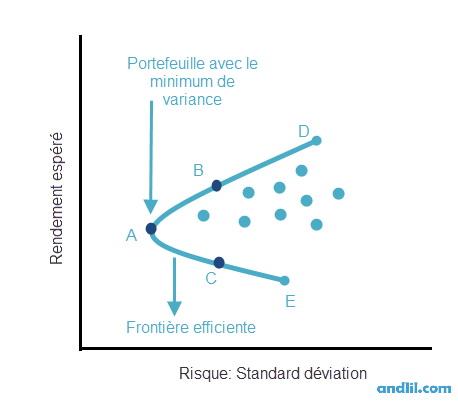
\includegraphics[scale=0.35]{images/frontiereEfficiente.png}   
	      \caption{Frontière efficiente - Problème de Markowitz}
	  \end{figure} 
      \end{column}
    \end{columns}
\end{frame}

\begin{frame}
    \frametitle{Ajout d'un actif sans risque} 
      \begin{figure}
	  \center
	  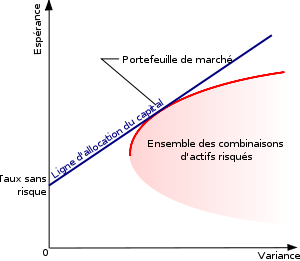
\includegraphics[scale=0.5]{images/cal.png}   
	  \caption{La CAL (Capital Allocation Line)}
      \end{figure} 
\end{frame}

